
\documentclass[a4paper,12pt]{article}

\usepackage{graphicx} % Required for inserting images
\usepackage{amsmath,amssymb,amsfonts}
\usepackage{subcaption}
% -----------------------
% Package Imports
% -----------------------

% Set page margins
\usepackage[a4paper, top=1in, bottom=0.8in, left=1.1in, right=0.8in]{geometry}

% Use Times New Roman font
\usepackage{times}

% Add page numbering
\pagestyle{plain}

% Enable graphics inclusion
\usepackage{graphicx}
\usepackage{float}
% Enable code listings
\usepackage{listings}
\usepackage{xcolor} % For customizing code colors
\setlength{\parindent}{0pt}




\begin{document}
	\section{Experiment No. 6}
	
	\section{Experiment Title }
Speed control of DC Shunt Motor
	\section{Objective}
	
	The objectives of this lab are as follows:
	\begin{itemize}
	\item To compare and contrast the armature control method and field control method for speed adjustment in DC shunt motors.
	\item To explore the effects of adjusting armature resistance on the armature current and consequently the motor speed.
	\item To investigate how field current adjustment influences the magnetic flux and motor speed, particularly in high-speed applications.
	\end{itemize}
	
	\section{Theory}
	
	\section*{Speed Control of DC Shunt Motor}
	
	The speed \( S \) of a DC shunt motor can be controlled by manipulating either the armature current \( I_a \) or the field flux \( \Phi \), as shown in the following formula:
	
	\[
	S = \frac{V_T - I_a R_a}{K \Phi}
	\]
	
	where:
	\begin{itemize}
		\item \( V_T \) is the terminal voltage supplied to the motor.
		\item \( I_a \) is the armature current, which flows through the armature winding.
		\item \( R_a \) is the resistance of the armature winding.
		\item \( K \) is a constant related to the motor’s construction.
		\item \( \Phi \) represents the magnetic flux per pole, which depends on the field current \( I_f \) flowing through the field winding.
	\end{itemize}
	
	\subsection*{Speed Control Methods}
	There are two main methods to control the speed of a DC shunt motor:
	
	\subsubsection*{1. Armature Control Method}
	This method involves changing \( I_a \), the armature current.
	\begin{itemize}
		\item By adjusting the resistance in the armature circuit, the voltage drop across \( R_a \) can be modified, thereby changing \( I_a \) and consequently the speed \( S \).
		\item This method is generally used when controlling the speed below the motor's rated speed.
	\end{itemize}
	
	\subsubsection*{2. Field Control Method}
	This method involves changing \( \Phi \) by adjusting \( I_f \), the field current.
	\begin{itemize}
		\item Decreasing \( \Phi \) (by reducing \( I_f \)) increases the speed since \( \Phi \) is in the denominator of the speed equation.
		\item This method is suitable for controlling the speed above the motor’s rated speed.
	\end{itemize}
	
	\section*{Field Control Method}
	
	The Field Control Method is used to achieve speeds above the motor’s base speed. This method controls the speed by adjusting the field current \( I_f \) that flows through the field winding, thereby changing the magnetic flux \( \Phi \). Field control is commonly used in high-speed applications such as centrifugal pumps, blowers, and pumps.
	

	The back EMF (\( E_b \)) in a DC motor is given by:
	\[
	E_b = K \Phi S
	\]
	where \( K \) is a constant, \( \Phi \) is the flux, and \( S \) is the speed.
	
	Rearranging this, we find that:
	\[
	S \propto \frac{1}{\Phi}
	\]
	This indicates that the motor speed is inversely proportional to the magnetic flux.
	
	To decrease \( \Phi \) and increase speed, a variable resistor \( R_f \) is added in series with the field winding. By increasing \( R_f \), we reduce \( I_f \) (the field current), which reduces \( \Phi \) (the flux).
	
	When the field resistance \( R_f \) is increased, the field current \( I_f \) decreases, reducing the magnetic flux \( \Phi \). Since speed is inversely related to flux \( \left( S \propto \frac{1}{\Phi} \right) \), a decrease in \( \Phi \) results in an increase in speed \( S \).
	
	Therefore, increasing the field resistance allows the motor to achieve speeds above its base speed.
		\begin{figure}[H]
		\centering
		\begin{subfigure}[t]{.48\textwidth}
			\centering
			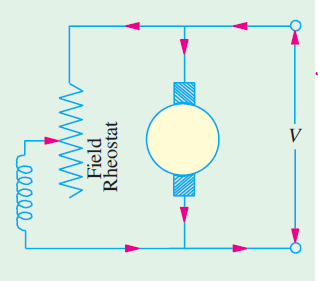
\includegraphics[width=0.9\linewidth]{Images/1}
			\caption{Field Control $I_f$ Method}
			\vspace{0.5cm}
		\end{subfigure}
		\hfill
		\begin{subfigure}[t]{.48\textwidth}
			\centering
			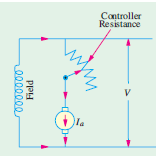
\includegraphics[width=.9\linewidth]{Images/2}
			\caption{ Armature Control $I_a$ Method }
		\end{subfigure}
		
		
	\end{figure}
	\section*{Armature Control Method}
	
	The current in the armature \( I_a \) is given by:
	
	\[
	I_a = \frac{V_T - E_b}{R_a + R_{ar}}
	\]
	
	where:
	\begin{itemize}
		\item \( E_b \) is the back EMF (Electromotive Force) generated by the rotation of the armature in the magnetic field.
		\item \( R_a \) is the internal resistance of the armature winding.
		\item \( R_{ar} \) is the external resistance added to the armature circuit for control purposes.
	\end{itemize}
	
	By adjusting \( R_{ar} \), we change the total resistance in the armature circuit, which affects \( I_a \) and subsequently the speed \( S \) of the motor.
	

	When \( R_{ar} \) is increased, the overall resistance in the armature circuit rises. This causes \( I_a \) to decrease, leading to a reduction in the torque \( T \), as:
	
	\[
	T \propto I_a
	\]
	
	Since torque \( T \) is proportional to the armature current \( I_a \), a decrease in torque means less force to drive the motor, resulting in a drop in the speed \( S \) of the motor.
	
	Therefore, increasing the armature resistance decreases the motor’s speed below its base speed.
	
	
	\newpage
	
	
	
	
	\section{Required Apparatus}
	\begin{enumerate}
		\item Variable Resistor (Ratings: Resistance: \( 5000 \, \Omega \), Current: \( 0.31 \, \text{A} \))
		\item Variable Resistor (Ratings: Resistance: \( 200 \, \Omega \), Current: \( 1.58 \, \text{A} \))
		\item Fixed DC Power Supply (Ratings: Voltage: \( 220 \, \text{V} \))
		\item DC Multimeter (Ratings: Voltage: \( 600 \, \text{V} \), Current: \( 20 \, \text{A} \))
	
		\item DC Motor (Ratings: Power: \( 300 \, \text{W} \), Voltage: \( 220 \, \text{V} \), Speed: \( 2500 \, \text{rpm} \))
		\item Tachogenerator (Ratings: Current: \( 0.07 \, \text{A} \) max, Speed: \( 5000 \, \text{rpm} \) max)
	\end{enumerate}
	
	\section{Circuit Diagrram}
	\begin{figure}[H]
		\centering
		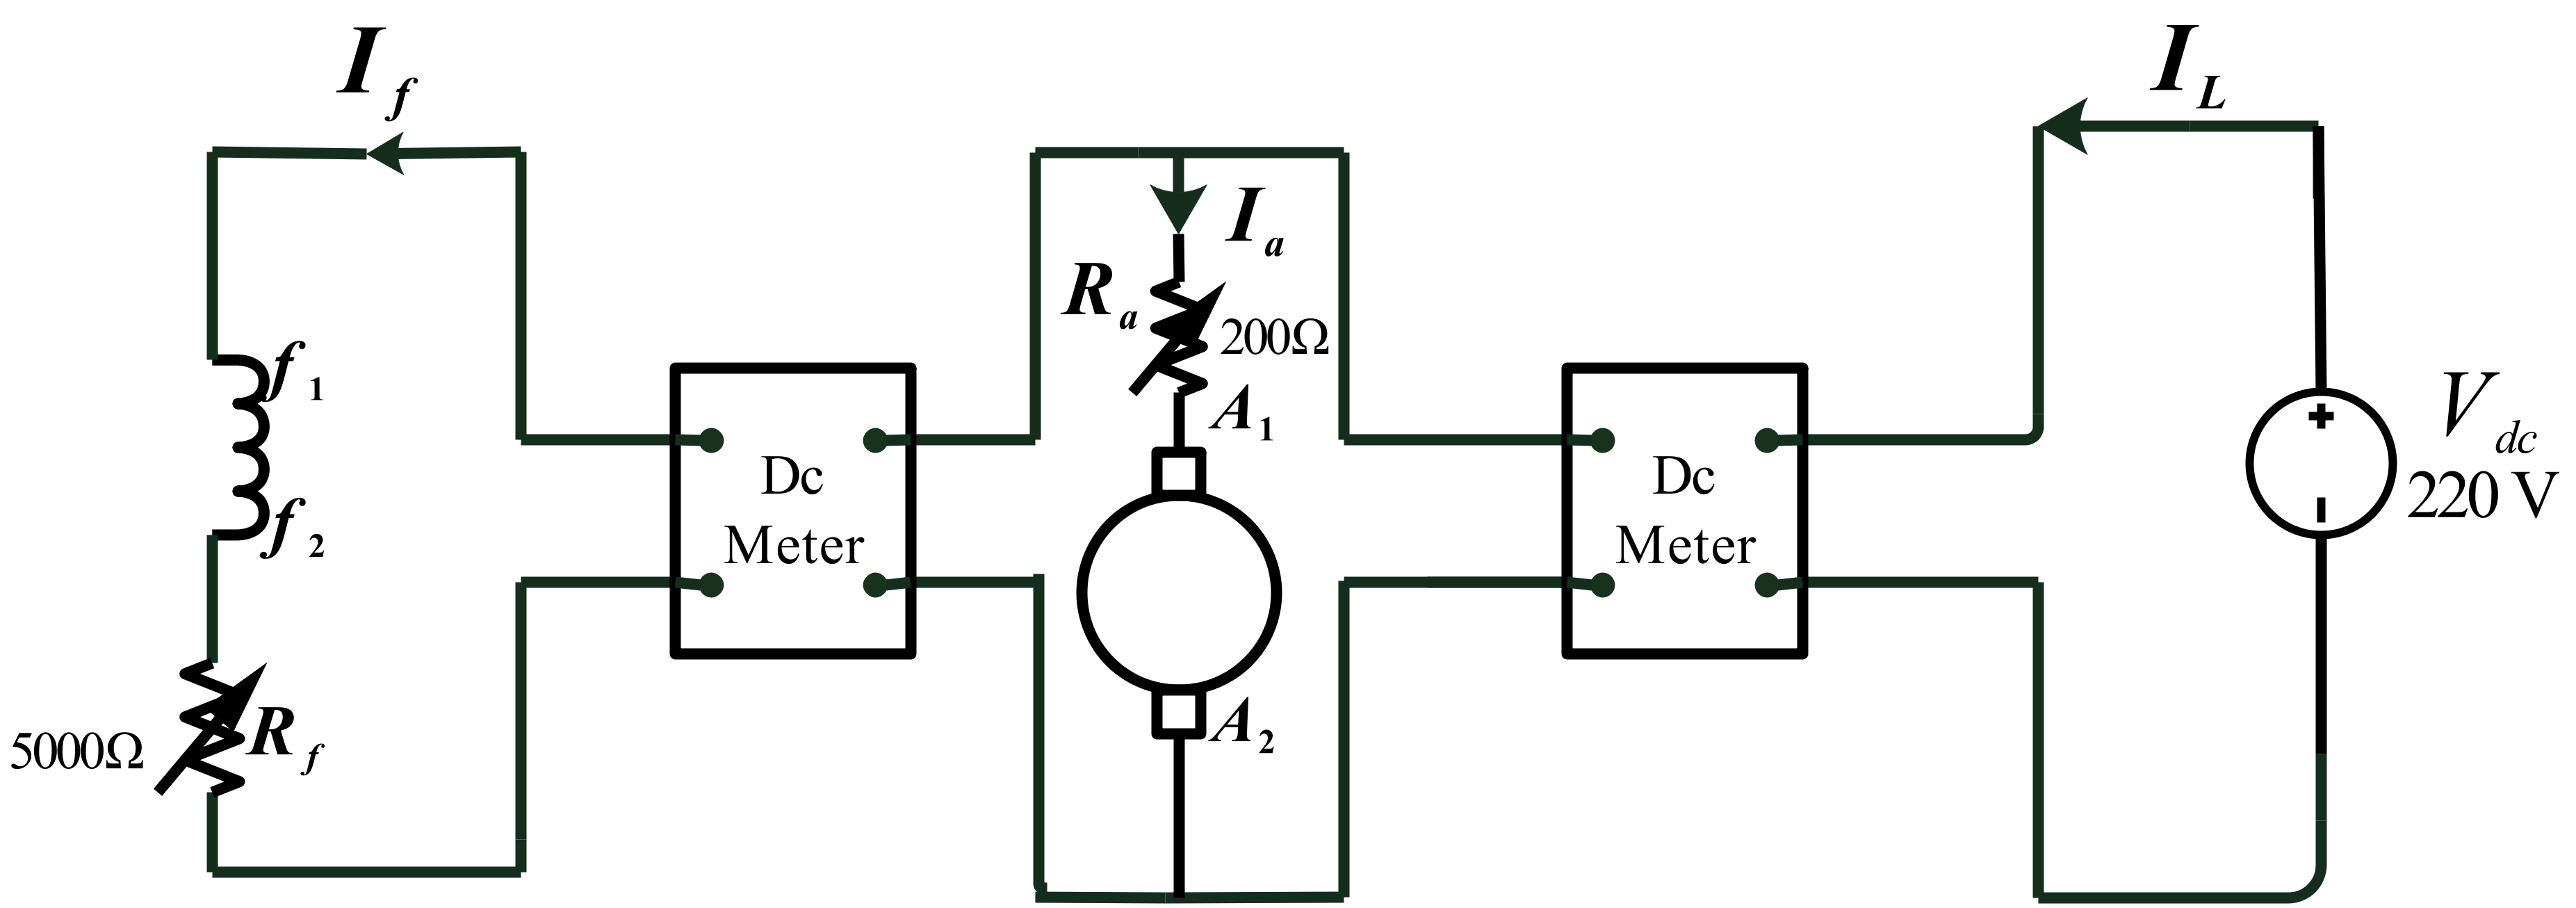
\includegraphics[width=1.1\textwidth]{Images/dcmotor}
		\caption{Required Circuit Diagram}
		
	\end{figure}
	
	
	
	
	
	\newpage
	\section{Data Table}

	\begin{table}[H]
\begin{subtable}[t]{1\textwidth} 
\centering

	\begin{tabular}{|c|c|c|}
		\hline
		\textbf{SI} & \textbf{\begin{tabular}[c]{@{}c@{}}Field Current,\\ $I_f (A)$\end{tabular}} & \textbf{\begin{tabular}[c]{@{}c@{}}Speed ,\\ $S (r.p.m)$\end{tabular}} \\ \hline
		1           & 0.1                                                                        & 2672                                                                 \\ \hline
		2           & 0.098                                                                      & 2693                                                                 \\ \hline
		3           & 0.095                                                                      & 2730                                                                 \\ \hline
		4           & 0.094                                                                      & 2744                                                                 \\ \hline
		5           & 0.092                                                                      & 2769                                                                 \\ \hline
		6           & 0.087                                                                      & 2813                                                                 \\ \hline
		7           & 0.084                                                                      & 2860                                                                 \\ \hline
		8           & 0.082                                                                      & 2892                                                                 \\ \hline
		9           & 0.08                                                                       & 2919                                                                 \\ \hline
		10          & 0.079                                                                      & 2936                                                                 \\ \hline
		11          & 0.077                                                                      & 2959                                                                 \\ \hline
		12          & 0.076                                                                      & 2975                                                                 \\ \hline
		13          & 0.074                                                                      & 2984                                                                 \\ \hline
		14          & 0.072                                                                      & 3001                                                                 \\ \hline
	\end{tabular}
\caption{Data table of Field current $(I_f)$ and Motor Speed $(S)$}
\vspace{1cm}
\end{subtable}

\begin{subtable}[t]{1\textwidth} 
	\centering
	\begin{tabular}{|c|c|c|}
	\hline
	\textbf{SI} & \textbf{\begin{tabular}[c]{@{}c@{}}Armature Current ,\\ $I_a (A) $\end{tabular}} & \textbf{\begin{tabular}[c]{@{}c@{}}Speed ,\\ $S (r.p.m)$\end{tabular}} \\ \hline
	1           & 0.326                                                                        & 2672                                                                 \\ \hline
	2           & 0.324                                                                        & 2644                                                                 \\ \hline
	3           & 0.322                                                                        & 2610                                                                 \\ \hline
	4           & 0.320                                                                        & 2587                                                                 \\ \hline
	5           & 0.317                                                                        & 2542                                                                 \\ \hline
	6           & 0.316                                                                        & 2504                                                                 \\ \hline
	7           & 0.315                                                                        & 2469                                                                 \\ \hline
	8           & 0.312                                                                        & 2438                                                                 \\ \hline
	9           & 0.311                                                                        & 2404                                                                 \\ \hline
	10          & 0.308                                                                        & 2356                                                                 \\ \hline
	11          & 0.307                                                                        & 2313                                                                 \\ \hline
	12          & 0.306                                                                        & 2290                                                                 \\ \hline
	13          & 0.305                                                                        & 2261                                                                 \\ \hline
	14          & 0.303                                                                        & 2221                                                                 \\ \hline
	15          & 0.301                                                                        & 2192                                                                 \\ \hline
\end{tabular}
\caption{Data table of Armature current $(I_a)$ and Motor Speed $(S)$}
\end{subtable}

\end{table}

	\section{Graph}
	\begin{figure}[H]
		\centering
		\begin{subfigure}[t]{1\textwidth}
			\centering
				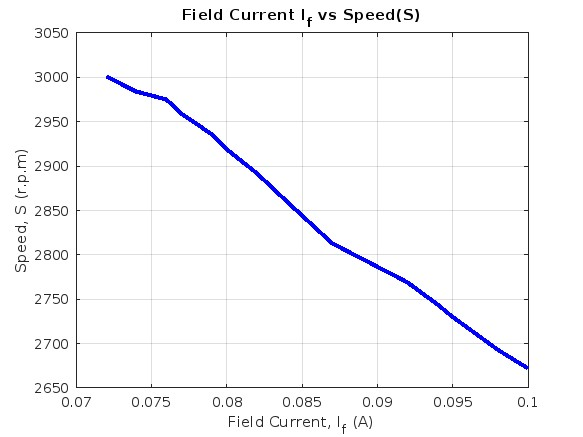
\includegraphics[width=0.9\linewidth]{Images/ifvsspeed}
			\caption{ $I_f$ vs. Speed Graph (S)}
			\vspace{0.5cm}
		\end{subfigure}
		
		\begin{subfigure}[t]{1\textwidth}
			\centering
			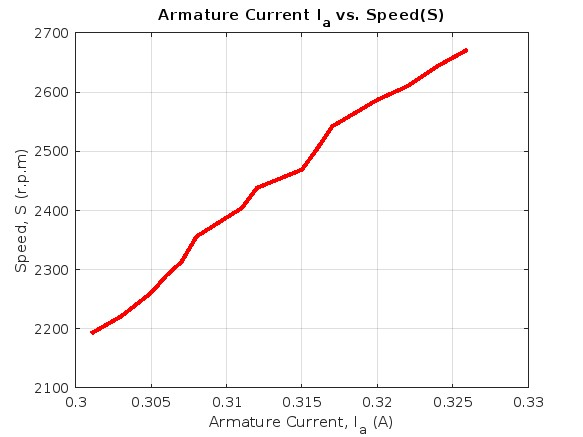
\includegraphics[width=0.9\linewidth]{Images/iavss}
			\caption{ $I_a$ vs. Speed Graph (S)}
		\end{subfigure}
		

	\end{figure}

\section{Discussion}

The experiment was conducted to investigate the speed control of a DC shunt motor. The relationship between the motor speed \( S \) and armature current \( I_a \) and field flux \( \Phi \) was analyzed. The relationship was described by the equation:

\[
S = \frac{V_T - I_a R_a}{K \Phi}
\]

It was observed that as the field resistance increased, \( I_f \) was decreased, which resulted in an increase in speed. Conversely, in the armature control method, the armature resistance was increased, causing \( I_a \) to decrease, leading to a reduction in speed. 
A fixed DC power supply of \( 220 \, \text{V} \) was provided for the experiment.
For careful motor startup, the armature resistance was initially maximized while the field resistance was minimized. After the motor started, the armature resistance was returned to a minimal setting to maintain the base speed.

\end{document}
